% Options for packages loaded elsewhere
\PassOptionsToPackage{unicode}{hyperref}
\PassOptionsToPackage{hyphens}{url}
%
\documentclass[
  10pt,
  a4paper,
]{article}
\usepackage{amsmath,amssymb}
\usepackage{iftex}
\ifPDFTeX
  \usepackage[T1]{fontenc}
  \usepackage[utf8]{inputenc}
  \usepackage{textcomp} % provide euro and other symbols
\else % if luatex or xetex
  \usepackage{unicode-math} % this also loads fontspec
  \defaultfontfeatures{Scale=MatchLowercase}
  \defaultfontfeatures[\rmfamily]{Ligatures=TeX,Scale=1}
\fi
\usepackage{lmodern}
\ifPDFTeX\else
  % xetex/luatex font selection
  \setmainfont[]{DejaVu Sans}
  \setmonofont[]{DejaVu Sans Mono}
\fi
% Use upquote if available, for straight quotes in verbatim environments
\IfFileExists{upquote.sty}{\usepackage{upquote}}{}
\IfFileExists{microtype.sty}{% use microtype if available
  \usepackage[]{microtype}
  \UseMicrotypeSet[protrusion]{basicmath} % disable protrusion for tt fonts
}{}
\makeatletter
\@ifundefined{KOMAClassName}{% if non-KOMA class
  \IfFileExists{parskip.sty}{%
    \usepackage{parskip}
  }{% else
    \setlength{\parindent}{0pt}
    \setlength{\parskip}{6pt plus 2pt minus 1pt}}
}{% if KOMA class
  \KOMAoptions{parskip=half}}
\makeatother
\usepackage{xcolor}
\usepackage[margin=19mm]{geometry}
\usepackage{longtable,booktabs,array}
\usepackage{calc} % for calculating minipage widths
% Correct order of tables after \paragraph or \subparagraph
\usepackage{etoolbox}
\makeatletter
\patchcmd\longtable{\par}{\if@noskipsec\mbox{}\fi\par}{}{}
\makeatother
% Allow footnotes in longtable head/foot
\IfFileExists{footnotehyper.sty}{\usepackage{footnotehyper}}{\usepackage{footnote}}
\makesavenoteenv{longtable}
\usepackage{graphicx}
\makeatletter
\def\maxwidth{\ifdim\Gin@nat@width>\linewidth\linewidth\else\Gin@nat@width\fi}
\def\maxheight{\ifdim\Gin@nat@height>\textheight\textheight\else\Gin@nat@height\fi}
\makeatother
% Scale images if necessary, so that they will not overflow the page
% margins by default, and it is still possible to overwrite the defaults
% using explicit options in \includegraphics[width, height, ...]{}
\setkeys{Gin}{width=\maxwidth,height=\maxheight,keepaspectratio}
% Set default figure placement to htbp
\makeatletter
\def\fps@figure{htbp}
\makeatother
\setlength{\emergencystretch}{3em} % prevent overfull lines
\providecommand{\tightlist}{%
  \setlength{\itemsep}{0pt}\setlength{\parskip}{0pt}}
\setcounter{secnumdepth}{-\maxdimen} % remove section numbering
\ifLuaTeX
\usepackage[bidi=basic]{babel}
\else
\usepackage[bidi=default]{babel}
\fi
\babelprovide[main,import]{french}
\ifPDFTeX
\else
\babelfont{rm}[]{DejaVu Sans}
\fi
% get rid of language-specific shorthands (see #6817):
\let\LanguageShortHands\languageshorthands
\def\languageshorthands#1{}
\usepackage{etoolbox}
\usepackage{microtype}
\usepackage{float}
\floatplacement{figure}{H}
\sloppy
\setlength{\emergencystretch}{5em}
\AtBeginEnvironment{longtable}{\small}
\ifLuaTeX
  \usepackage{selnolig}  % disable illegal ligatures
\fi
\IfFileExists{bookmark.sty}{\usepackage{bookmark}}{\usepackage{hyperref}}
\IfFileExists{xurl.sty}{\usepackage{xurl}}{} % add URL line breaks if available
\urlstyle{same}
\hypersetup{
  pdftitle={Un Lego réutilisable et un premier certificat complet},
  pdfauthor={Vincent P. P. NOËL - dossier de recherche, rédaction assistée},
  pdflang={fr-FR},
  hidelinks,
  pdfcreator={LaTeX via pandoc}}

\title{Un Lego réutilisable et un premier certificat complet}
\usepackage{etoolbox}
\makeatletter
\providecommand{\subtitle}[1]{% add subtitle to \maketitle
  \apptocmd{\@title}{\par {\large #1 \par}}{}{}
}
\makeatother
\subtitle{Programme Riemann - V6.46 - Document 71}
\author{Vincent P. P. NOËL - dossier de recherche, rédaction assistée}
\date{12 octobre 2026}

\begin{document}
\maketitle

{
\setcounter{tocdepth}{2}
\tableofcontents
}
\hypertarget{faisabilituxe9-une-construction-exuxe9cutuxe9e}{%
\section{1. Faisabilité : une construction
exécutée}\label{faisabilituxe9-une-construction-exuxe9cutuxe9e}}

Un premier assemblage complet est réalisé. Il porte sur \textbf{tous les
tests admissibles} d'un espace de dimension infinie, avec le premier 2
réellement présent. Ce résultat dépasse la vérification d'une
compression matricielle.

\textbf{Théorème local certifié.} Pour tout \(0<S\le347/1000\), et tout
\(f\in X_S\) admissible dans le domaine de la forme de V644--V645, \[
\boxed{Q_W(f)\ge\frac1{25}\|f\|_2^2,
\qquad Q_W(f)\ge\frac1{200}R(f),
\qquad\|f\|_2^2\le\frac3{20}R(f).}
\] Ici \(R=\|f\|_2^2+\mathcal E(f)\). La preuve combine les lemmes
K1--K6 ci-dessous avec cinq inégalités rationnelles effectivement
encadrées. La marge massique plus précise du journal est supérieure à
0,0479 ; le théorème conserve des constantes simples et prudentes. Il
n'utilise ni zéros, ni RH, ni les anciennes quadratures archimédiennes
exploratoires.

La positivité est acquise sur une famille \textbf{bornée} de supports.
Aucune exhaustion vers l'infini n'est obtenue. Les réponses à S=0,348 et
S=1/2 restent indéterminées pour cet assemblage, sans témoin négatif de
Q\_W.

Le Lego est constitué de preuves analytiques, d'encadrements numériques
et de raccords typés. Il n'est pas un assistant de preuve formelle : les
données d'une brique arbitraire ne sont pas authentifiées par la seule
présence d'un label. Les constructeurs, les erreurs et les lemmes
doivent être contrôlés ensemble. La nouveauté annoncée est interne au
programme ; aucune priorité dans la littérature n'est revendiquée.

\hypertarget{les-piuxe8ces-et-leurs-raccords}{%
\section{2. Les pièces et leurs
raccords}\label{les-piuxe8ces-et-leurs-raccords}}

\begin{longtable}[]{@{}
  >{\raggedright\arraybackslash}p{(\columnwidth - 4\tabcolsep) * \real{0.3333}}
  >{\raggedright\arraybackslash}p{(\columnwidth - 4\tabcolsep) * \real{0.3333}}
  >{\raggedright\arraybackslash}p{(\columnwidth - 4\tabcolsep) * \real{0.3333}}@{}}
\toprule\noalign{}
\begin{minipage}[b]{\linewidth}\raggedright
Pièce
\end{minipage} & \begin{minipage}[b]{\linewidth}\raggedright
Image pour apprendre
\end{minipage} & \begin{minipage}[b]{\linewidth}\raggedright
Garantie et raccord
\end{minipage} \\
\midrule\noalign{}
\endhead
\bottomrule\noalign{}
\endlastfoot
Domaine & Une boîte de taille S & Support, moments, régularité, forme,
norme R et unité \\
Moule P & Le moule fabrique une pièce admissible & Pψ respecte les deux
moments ; origine V644 \\
Projection & Retirer ce que les balances ne lisent pas & Le même Gram
sert aux sources et aux fréquences \\
Parité & Deux tiroirs qui ne se mélangent pas & Découplage exact
pair/impair pour énergie et premiers \\
Couches & Plusieurs règles mesurent la même pièce & Une somme finie
minore l'énergie sur tous les tests \\
Bord & Les attaches au bord coûtent de l'énergie & Le potentiel pénalise
les bandes du couplage premier \\
Assembleur & Vérifier tous les raccords & Mélange convexe, marge,
contrôle R et statut \\
Inclusion & Une petite boîte entre dans la grande & Tous S≤S₀ héritent
de la preuve sur X\_S₀ \\
\end{longtable}

Les tests, les annihilateurs et les sources sont des objets distincts.
Les tests et sources portent l'unité fictive \(A_{\rm amp}\) ; les
formes, potentiels appliqués à une masse et Grams portent
\(A_{\rm amp}^2\). S et les fréquences sont logarithmiques sans
dimension. Les constantes λ, μ, β et α sont sans dimension.

Un port contient S, la forme exacte et son éventuel décalage massique,
les annihilateurs, la norme et l'unité. Deux briques de supports, formes
ou unités différents ne se raccordent pas. Une vérification sur des
échantillons ne porte pas le statut « tous les tests ». Un certificat
borné ne reçoit pas le statut « tous les supports jusqu'à l'infini ».

\hypertarget{cadre-commun-et-conventions}{%
\section{3. Cadre commun et
conventions}\label{cadre-commun-et-conventions}}

Sur \(I_S=[-S,S]\), prolonger f par zéro et imposer \[
\int f(x)\cosh(x/2)dx=\int f(x)\sinh(x/2)dx=0.
\] Ces deux conditions sont équivalentes aux moments exponentiels de
V644. Précisément, X\_S est le sous-espace des fonctions L² portées par
I\_S, ayant ces deux moments nuls et une énergie finie. R(f) est le
carré de la norme énergétique : \(\|f\|_R=\sqrt{R(f)}\). On utilise \[
\mathcal E(f)=\int_0^\infty w(t)\|U_tf-f\|_2^2dt,
\quad w(t)=\frac{e^{-t/2}}{1-e^{-2t}},\quad
C_0=\log(8\pi)+\gamma_E+\frac\pi2.
\] \[
Q_W(f)=\mathcal E(f)-C_0\|f\|_2^2
-2\sum_{p^m\le e^{2S}}\frac{\log p}{p^{m/2}}\Re h_f(m\log p).
\] La Fourier est unitaire, avec exponentielle e⁻ⁱᵗˣ et facteur
\((2\pi)^{-1/2}\). Son multiplicateur énergétique est \[
a(T)=\sum_{n\ge0}\frac{2T^2}{b_n(b_n^2+T^2)},\qquad b_n=2n+\tfrac12.
\] Il est croissant, nul en 0. Chaque terme est positif. La
représentation par digamma, cohérente avec {[}NIS10{]}, sert à une
comparaison ponctuelle indépendante ; la preuve numérique utilise la
série positive et son reste.

Le cadre de Weil et les projections de coupure sont rapprochés de
{[}CC21{]}. Le résultat de ce document est démontré directement dans nos
conventions ; la lecture bibliographique ne sert pas à supposer son
signe.

\hypertarget{k1---une-projection-ouvre-deux-portes}{%
\section{4. K1 - Une projection ouvre deux
portes}\label{k1---une-projection-ouvre-deux-portes}}

Soit W un sous-espace fini de L²(I), de base w\_j et de Gram G
strictement positif. La projection \(\Pi_W\) possède deux usages.

\textbf{Sources.} Pour de vraies sources fortes \(k_i\in L^2(I)\), poser
\(K_{ij}=\langle k_i,k_j\rangle\), \(B_{ji}=\langle w_j,k_i\rangle\).
Alors \[
C_{\rm opt}=\operatorname{Gram}((I-\Pi_W)k_i)=K-B^*G^{-1}B.
\] Pour toute correction \(p_i\in W\), l'orthogonalité donne \[
\operatorname{Gram}(k_i-p_i)=C_{\rm opt}
+\operatorname{Gram}(\Pi_Wk_i-p_i)\succeq C_{\rm opt}.
\] La projection améliore donc la matrice entière en ordre de Loewner,
avec les couplages, pas seulement ses diagonales. Pour l'usage Schur, W
doit annihiler la queue correspondante. Les intégrations, G et son
inversion restent à encadrer lorsque les sources sont numériques. Le
programme implémente ici l'algèbre rationnelle sur un exemple de Gram
cohérent ; il ne prétend pas avoir certifié toutes les sources de ζ.

\textbf{Fréquences.} Pour f∈W⊥, Cauchy--Schwarz donne \[
|\widehat f(t)|^2\le\frac{\|f\|_2^2}{2\pi}
\|(I-\Pi_W)e^{itx}\|_2^2.
\] Le même G⁻¹ retire donc aussi la part fréquentielle interdite. C'est
le premier coup double. La contraction de \(I-\Pi_W\) conserve les
majorants d'erreur L² des sources ; les erreurs de calcul de la
projection doivent s'ajouter. □

\hypertarget{k2---la-parituxe9-donne-des-traces-plus-fines}{%
\section{5. K2 - La parité donne des traces plus
fines}\label{k2---la-parituxe9-donne-des-traces-plus-fines}}

Prendre \(W=\operatorname{span}\{\cosh(x/2),\sinh(x/2)\}\). La réflexion
commute avec les déplacements symétrisés et l'énergie. Elle préserve les
moments ; f=f\_pair+f\_impair découple toutes les formes. Les deux
normes du Gram sont \[
g_+=S+\sinh S,\qquad g_-=\sinh S-S>0.
\] Poser \[
z_S(t)=\frac{2\sinh((1/2+it)S)}{1/2+it},\quad
b_c(t)=\Re z_S(t),\quad b_s(t)=\Im z_S(t).
\] Les diagonales projetées sont \[
d_+(t)=S+\frac{\sin(2tS)}{2t}-\frac{b_c(t)^2}{g_+},
\] \[
d_-(t)=S-\frac{\sin(2tS)}{2t}-\frac{b_s(t)^2}{g_-}.
\] Les valeurs en 0 sont définies par continuité. Ces expressions sont
les normes carrées projetées de cos(tx) et sin(tx) ; elles sont non
négatives. Pour un test de la parité correspondante, \[
\int_{-T}^T|\widehat f(t)|^2dt
\le\min(1,\kappa_\pm(T))\|f\|_2^2,
\quad \kappa_\pm(T)=\frac1\pi\int_0^T d_\pm(t)dt.
\] La borne résulte de K1 puis de l'intégration. Séparer les parités
remplace la trace totale par deux traces plus petites et conserve le
contrôle des termes croisés qui doivent être nuls : deuxième coup
double. □

\hypertarget{k3---cumuler-les-couches-sans-quadrature-infinie}{%
\section{6. K3 - Cumuler les couches, sans quadrature
infinie}\label{k3---cumuler-les-couches-sans-quadrature-infinie}}

Pour \(0=T_0<T_1<\cdots<T_m\), la monotonie de a donne, point par point,
\[
a(t)\ge\sum_{j=1}^m[a(T_j)-a(T_{j-1})]\,\mathbf1_{|t|\ge T_j}.
\] Plancherel et K2 donnent donc \[
\mathcal E(f)\ge\lambda_\pm\|f\|_2^2,
\] \[
\lambda_\pm=\sum_{j=1}^m
[a(T_j)-a(T_{j-1})]\,[1-\min(1,\kappa_\pm(T_j))].
\] Le minimum des deux λ couvre tout f admissible, même complexe. La
fréquence au-delà du dernier seuil n'est pas supprimée : le dernier
étage reste un minorant sur toute cette queue. Aucun reste d'une
quadrature énergétique infinie n'est oublié. □

\textbf{Encadrement exécuté.} m=32, T\_j=3j/8. Chaque intégrale de κ est
calculée par milieux avec h=3/(8·256). Si v=(I−Π)cos(tx) ou sin(tx), \[
|\partial_t\|v\|^2|\le2\|v\|\|v'\|
\le\frac{4S^2}{\sqrt3}\le4S^2=:M.
\] La contraction de la projection et \(\int_{-S}^Sx^2dx=2S^3/3\)
justifient la borne. L'erreur totale des milieux jusqu'à T vaut au plus
MTh/4, puis on divise par π. Ce terme d'erreur est ajouté au majorant κ,
jamais retranché.

Pour chaque incrément, on somme les n\textless64 en fractions
rationnelles avant les transcendantes. Pour n≥64, l'incrément est \[
\frac{2b_n(T_j^2-T_{j-1}^2)}
{(b_n^2+T_j^2)(b_n^2+T_{j-1}^2)}.
\] Il décroît lorsque b\_n≥T\_j. La comparaison série/intégrale minore
sa somme par \[
\frac12\log\frac{b_{64}^2+T_j^2}{b_{64}^2+T_{j-1}^2}.
\] Ajouter le premier terme du reste fournit un majorant. Tous les
calculs élémentaires utilisent des intervalles binaires à 160 bits. Les
extrémités orientées alimentent ensuite l'algèbre rationnelle exacte.

\hypertarget{k4---le-bord-paie-pruxe9cisuxe9ment-les-attaches-premiuxe8res}{%
\section{7. K4 - Le bord paie précisément les attaches
premières}\label{k4---le-bord-paie-pruxe9cisuxe9ment-les-attaches-premiuxe8res}}

Définir \[
J(d)=\int_d^\infty w(t)dt
=\frac12\log\frac{1+e^{-d/2}}{1-e^{-d/2}}+\arctan(e^{-d/2}),\quad d>0.
\] Dans l'énergie des déplacements, les interactions avec l'extérieur de
I donnent \[
\mathcal E(f)\ge\int_I V_S(x)|f(x)|^2dx,
\quad V_S(x)=J(S-x)+J(S+x).
\] \textbf{Preuve.} Séparer les paires de points tous deux dans I des
paires dont un point est hors I, où f vaut zéro. Le premier terme est
une intégrale de différences carrées non négative ; le second est
exactement le potentiel annoncé. Tonelli s'applique aux termes positifs,
même pour le domaine de forme. Le potentiel minimal vaut 2J(S), puisque
J est convexe. □

Pour S₀=347/1000, a=log2 et δ=2S₀−a, on a \[
0<\delta<S_0,\qquad a<2S_0<\log3<2a.
\] Le seul terme premier est 2. Son couplage se produit entre les deux
bandes \([-S_0,S_0-a]\) et \([-S_0+a,S_0]\), de largeur δ. Si M\_bord
est la masse totale dans ces bandes disjointes et w₂=log2/√2, \[
Q_{\rm pr}(f)\le w_2M_{\rm bord}(f).
\] Cela suit de \(2\Re(u\bar v)\le|u|^2+|v|^2\). Sur les bandes, le
potentiel est au moins J(δ)+J(a). Si v₀,v₁ sont deux planchers
certifiés, respectivement hors bandes et dans les bandes, alors \[
\mathcal E(f)\ge v_0\|f\|^2+(v_1-v_0)M_{\rm bord}(f).
\] La différence v₁−v₀ concerne les \textbf{planchers choisis} ; elle
n'est pas présentée comme une minoration de la différence des potentiels
exacts. Le confinement qui crée le couplage premier crée également son
coût énergétique : troisième coup double. □

\hypertarget{k5---lassembleur-fournit-une-marge-lisible}{%
\section{8. K5 - L'assembleur fournit une marge
lisible}\label{k5---lassembleur-fournit-une-marge-lisible}}

Avec \(\mathcal E\ge\lambda\|f\|^2\), prendre α∈{[}0,1{]} tel que
\(\alpha(v_1-v_0)\ge w_2\). Un mélange des deux minorations de la même
énergie donne \[
Q_W(f)\ge[(1-\alpha)\lambda+\alpha v_0-C_0]\|f\|^2.
\] Le programme choisit α=w₂\_upper/(v₁\_lower−v₀\_lower) quand ce
nombre est ≤1. Si la marge n'est pas positive, la réponse est
\textbf{indéterminée} : la forme exacte peut encore être positive. Une
norme première indépendante maximale échoue ici ; le mélange garde la
relation entre coût énergétique et attaches.

Le journal prouve les cinq inégalités rationnelles simples \[
\lambda\ge\frac{231}{40},\quad v_0\ge\frac{769}{200},
\quad v_1\ge\frac{1627}{250},
\] \[
C_0\le\frac{5373}{1000},\qquad w_2\le\frac{491}{1000}.
\] Prendre α=3/16. Son paiement de bord dépasse w₂\_upper. L'algèbre
exacte donne \[
c=(1-\alpha)\frac{231}{40}+\alpha\frac{769}{200}
-\frac{5373}{1000}=\frac{321}{8000}>\frac1{25}.
\] Cette preuve de signe tient dans cinq encadrements et une égalité
rationnelle. Le contrôle d'erreur des couches garantit la première
inégalité ; les quatre autres utilisent les fonctions élémentaires de K4
et l'encadrement de γ\_E. □

\hypertarget{k6---deuxiuxe8me-usage-contrat-r-et-couverture-bornuxe9e}{%
\section{9. K6 - Deuxième usage : contrat R et couverture
bornée}\label{k6---deuxiuxe8me-usage-contrat-r-et-couverture-bornuxe9e}}

Poser m=\textbar\textbar f\textbar\textbar² et L=C₀\_upper+w₂\_upper. On
a simultanément \(Q_W\ge c m\) et \(Q_W\ge\mathcal E-Lm\). Leur mélange,
avec poids \(c/(c+L+1)\) sur la seconde, donne \[
Q_W\ge\frac{c}{c+L+1}(\mathcal E+m)=\mu R.
\] De \(\mathcal E\ge\lambda m\), on obtient
\(m\le R/(1+\lambda)=\beta R\). Les constantes rationnelles de K5
impliquent μ\textgreater1/200 et β\textless3/20. Le même assemblage
fournit donc signe et contrats directement utilisables dans Schur. La
tête peut être nulle : tout X\_S₀ possède déjà une marge coercive. □

Pour S≤S₀, l'extension par zéro identifie X\_S à un sous-espace de X\_S₀
: support, moments, R et Q\_W globaux restent les mêmes. Toutes les
inégalités s'y restreignent. Aucun test de monotonie numérique des
algorithmes λ(S) n'est nécessaire. Cette preuve couvre une infinité de
supports, mais seulement dans un intervalle borné. L'agrandissement
au-delà de S₀ ajoute de nouvelles directions.

\hypertarget{k7---contruxf4le-nuxe9gatif-et-garde-contre-les-faux-raccords}{%
\section{10. K7 - Contrôle négatif et garde contre les faux
raccords}\label{k7---contruxf4le-nuxe9gatif-et-garde-contre-les-faux-raccords}}

Le contrôle négatif modifie volontairement la forme :
Q\_η=Q\_W−η\textbar\textbar f\textbar\textbar². Pour la graine
polynomiale f=P(1−x²/S₀²)⁴, les masses sont rationnelles et \[
Q_W(f)\le\frac{131}{8}\|f'\|^2-\frac{25}{6}\|f\|^2
+w_{2,\rm upper}\|f\|^2.
\] Choisir un entier η strictement supérieur à ce quotient majoré
produit un vrai témoin négatif encadré de Q\_η. L'assembleur ne certifie
pas cette forme. Cela teste sa sensibilité à une perturbation, sans
constituer un contre-exemple à RH. Le port distingue Q\_W de Q\_η et
porte la valeur exacte de η. □

Le code refuse supports ou unités incompatibles, formes non prises en
charge, décalages massiques incohérents, erreurs de rôle et couverture
par seuls échantillons. L'algèbre de projection refuse un Gram singulier
ou un Gram joint incompatible. L'inversion presque singulière reste une
difficulté réelle pour des bases polynomiales/exponentielles plus
grandes.

\hypertarget{exuxe9cution-et-portuxe9e-des-ruxe9sultats}{%
\section{11. Exécution et portée des
résultats}\label{exuxe9cution-et-portuxe9e-des-ruxe9sultats}}

\begin{longtable}[]{@{}llll@{}}
\toprule\noalign{}
S & λ inférieur encadré & marge massique de l'assembleur & statut \\
\midrule\noalign{}
\endhead
\bottomrule\noalign{}
\endlastfoot
347/1000 & 5.77594295 & 0.04798711 & certifié sur tous les tests \\
87/250 & 5.77388642 & -0.05789517 & indéterminé \\
1/2 & 5.43323013 & poids convexe \textgreater{} 1 & indéterminé \\
\end{longtable}

Les supports et le maillage ont été sélectionnés après exploration
constructive et critique. Le protocole a été figé avant ces évaluations
par intervalles ; aucune découverte du signe n'est présentée comme une
prévision indépendante. Le journal sauvegarde les bornes binaires des
couches, leur erreur de milieux, les incréments positifs et les marges
rationnelles. Les deux lectures ont recoupé les facteurs et les
domaines. Une quadrature ponctuelle indépendante confirme les
orientations, mais elle n'est pas la source du certificat.

Une brique plus élémentaire, par disjonction des supports des
translations, donne déjà un certificat complet pour S≤1/32 sans premier.
Le résultat S₀ franchit log2/2 et rencontre effectivement le premier 2.
Il reste très local.

\begin{figure}
\centering
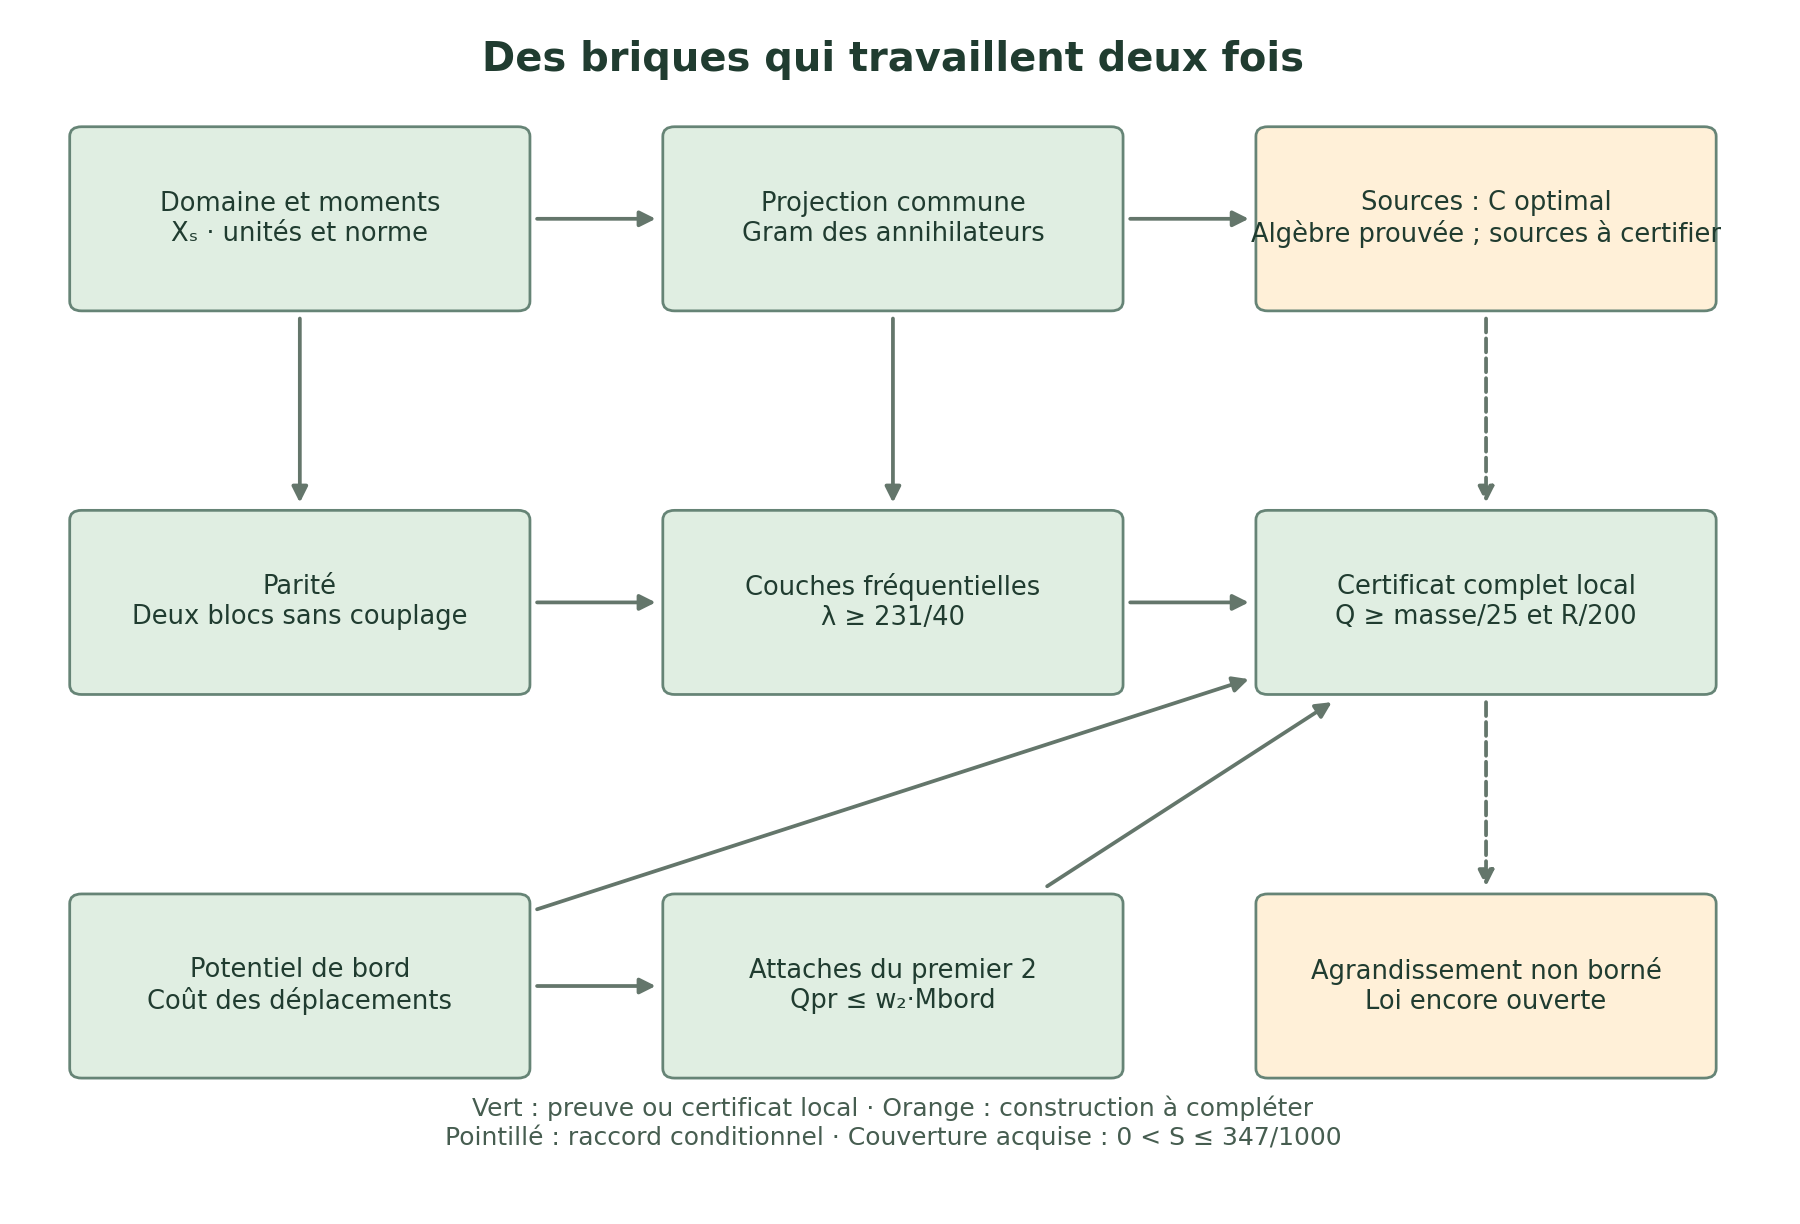
\includegraphics{71_GRAPHE_LEGO.png}
\caption{Les raccords du Lego et leurs limites.}
\end{figure}

\hypertarget{quatre-portes-creusuxe9es-diagnostic-dun-opuxe9rateur-conjoint}{%
\section{12. Quatre portes creusées : diagnostic d'un opérateur
conjoint}\label{quatre-portes-creusuxe9es-diagnostic-dun-opuxe9rateur-conjoint}}

Le premier2 peut aussi être conservé directement en Fourier, sans
séparer son poids de sa phase. Avec la Fourier unitaire et un seul
premier, \[
Q_W(f)=\int_{\mathbb R}[b(\tau)-C_0-2w_2]|\widehat f(\tau)|^2d\tau,
\] \[
b(\tau)=a(\tau)+2w_2[1-\cos(\tau\log2)].
\] La traduction est exacte. L'enveloppe croissante
\(g(T)=\inf_{\tau\ge T}b(\tau)\) donne un minorant, mais peut perdre
beaucoup des oscillations en créant des plateaux. Une grille ponctuelle
ne certifie pas cet infimum. Des planchers peuvent former une fonction
en escalier minorante, à condition de les monotoniser ; leurs
différences ne sont pas supposées être des minorants des incréments
exacts de g.

Une seconde voie conserve les sous-niveaux
\(\Omega_u=\{\tau:b(\tau)<u\}\), qui sont des unions de bandes. La même
projection de K2 donne \[
\kappa_{\pm,b}(u)=\frac1\pi\int_{\tau>0,\ b(\tau)<u}d_\pm(\tau)d\tau.
\] L'intégration des couches en valeur u, plutôt qu'en fréquence T,
fournit une cible de minoration énergétique par
\(\int_0^\infty[1-\min(1,\kappa_{\pm,b}(u))]du\). Elle garde davantage
de la phase du premier et réutilise le Gram déjà construit.

Le script de diagnostic a été réellement exécuté à 40 000 puis 80 000
points, jusqu'à la fréquence100. Il utilise des évaluations ponctuelles
et des intégrales discrètes : \textbf{aucune de ces nouvelles marges
n'est certifiée}.

\begin{longtable}[]{@{}
  >{\raggedright\arraybackslash}p{(\columnwidth - 6\tabcolsep) * \real{0.2500}}
  >{\raggedright\arraybackslash}p{(\columnwidth - 6\tabcolsep) * \real{0.2500}}
  >{\raggedright\arraybackslash}p{(\columnwidth - 6\tabcolsep) * \real{0.2500}}
  >{\raggedright\arraybackslash}p{(\columnwidth - 6\tabcolsep) * \real{0.2500}}@{}}
\toprule\noalign{}
\begin{minipage}[b]{\linewidth}\raggedright
S
\end{minipage} & \begin{minipage}[b]{\linewidth}\raggedright
séparation géométrique
\end{minipage} & \begin{minipage}[b]{\linewidth}\raggedright
enveloppe monotone
\end{minipage} & \begin{minipage}[b]{\linewidth}\raggedright
sous-niveaux joints
\end{minipage} \\
\midrule\noalign{}
\endhead
\bottomrule\noalign{}
\endlastfoot
347/1000 & -0.02954653 & -0.23163981 & 0.03765804 \\
3/8 & -0.10763132 & -0.29955459 & -0.03842748 \\
1/2 & -0.39801074 & -0.57750979 & -0.18668185 \\
\end{longtable}

À S=1/2, les sous-niveaux améliorent nettement le budget exploratoire,
mais celui-ci reste négatif. Cela indique une insuffisance de ce
minorant, pas un témoin négatif de Q\_W. L'accord des deux résolutions
mesure une stabilité, pas une erreur prouvée. Une certification
demanderait les frontières des sous-niveaux, les intégrales et la queue
; b≥a pourrait exclure celle-ci.

La concentration peut encore être affinée par
\(\|K\|\le\min(\operatorname{tr}K,\sqrt{\operatorname{tr}K^2})\) pour
l'opérateur positif projeté. Ce raccord réutiliserait encore le Gram,
mais sa double intégrale n'a pas été exécutée dans ce diagnostic
reproductible.

\hypertarget{les-prochaines-constructions-conserver-les-coups-doubles}{%
\section{13. Les prochaines constructions : conserver les coups
doubles}\label{les-prochaines-constructions-conserver-les-coups-doubles}}

\begin{longtable}[]{@{}
  >{\raggedright\arraybackslash}p{(\columnwidth - 4\tabcolsep) * \real{0.3333}}
  >{\raggedright\arraybackslash}p{(\columnwidth - 4\tabcolsep) * \real{0.3333}}
  >{\raggedright\arraybackslash}p{(\columnwidth - 4\tabcolsep) * \real{0.3333}}@{}}
\toprule\noalign{}
\begin{minipage}[b]{\linewidth}\raggedright
Porte
\end{minipage} & \begin{minipage}[b]{\linewidth}\raggedright
Acquis dans cette étape
\end{minipage} & \begin{minipage}[b]{\linewidth}\raggedright
Travail restant
\end{minipage} \\
\midrule\noalign{}
\endhead
\bottomrule\noalign{}
\endlastfoot
Sources et fréquences & Même projection, réduction Loewner et
concentration & Sources fortes et erreurs L² réelles pour les têtes non
coercives \\
Énergie et premiers & Coût de bord paie le premier 2 sur S≤0,347 &
Estimation jointe plus fine quand les bandes s'élargissent ou se
recouvrent \\
Queue et tête & Contrat R sur tout X\_S₀, tête nulle & Représentation
praticable pour des supports plus grands \\
Couverture & Tous les supports d'une famille bornée & Loi de transport
ou autre mécanisme atteignant S\_n→∞ \\
Convergence & Domaines et gardes explicites & Norme de graphe si une
approximation de sources/opérateurs la requiert \\
\end{longtable}

La priorité est d'affiner \textbf{l'opérateur conjoint énergie moins
déplacements premiers}, plutôt que d'augmenter une tête brute. Des
concentrations par opérateur, au lieu de la seule trace, et des
potentiels par cellules pourraient conserver davantage de relations
utiles. Les projections devront améliorer simultanément les contrôles
fréquentiels et les résidus de sources.

La première brique complète existe maintenant. La règle d'agrandissement
reste le verrou : réussir un support plus grand par le même mécanisme,
puis démontrer ce qui se transporte sur une famille non bornée. RH, les
collisions historiques et les paramètres complexes des autres familles
restent ouverts dans leur portée.

\hypertarget{ruxe9fuxe9rences}{%
\subsection{Références}\label{ruxe9fuxe9rences}}

Format : {[}clé{]} auteurs, \emph{titre}, publication, lien. Fiches
complètes et état de vérification : document 42 (registre des sources).

\begin{itemize}
\tightlist
\item
  {[}CC21{]} A. Connes, C. Consani. \emph{Weil positivity and Trace
  formula, the archimedean place}. PDF auteur daté du 4 juillet 2021 ;
  arXiv:2006.13771.
  \url{https://alainconnes.org/wp-content/uploads/Selecta.pdf} ---
  partiellement vérifié
\item
  {[}NIS10{]} F. W. J. Olver, D. W. Lozier, R. F. Boisvert, C. W. Clark
  (éd.). \emph{NIST Digital Library of Mathematical Functions, chapitre
  5, équation 5.9.16}. NIST DLMF, édition en ligne (2010).
  \url{https://dlmf.nist.gov/5.9\#E16} --- vérifié en ligne
\end{itemize}

\end{document}
